
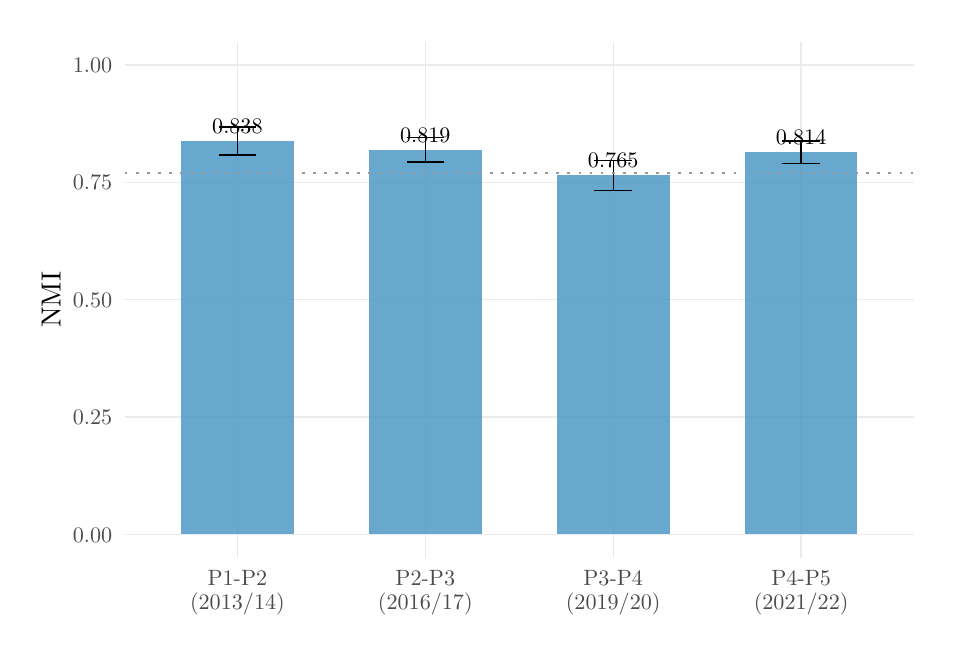
\begin{tikzpicture}[x=1pt,y=1pt]
\definecolor{fillColor}{RGB}{255,255,255}
\path[use as bounding box,fill=fillColor,fill opacity=0.00] (0,0) rectangle (325.21,216.81);
\begin{scope}
\path[clip] (  0.00,  0.00) rectangle (325.21,216.81);
\definecolor{fillColor}{RGB}{255,255,255}

\path[fill=fillColor] ( -0.00,  0.00) rectangle (325.21,216.81);
\end{scope}
\begin{scope}
\path[clip] ( 35.05, 25.20) rectangle (320.21,211.81);
\definecolor{drawColor}{gray}{0.92}

\path[draw=drawColor,line width= 0.5pt,line join=round] ( 35.05, 33.69) --
	(320.21, 33.69);

\path[draw=drawColor,line width= 0.5pt,line join=round] ( 35.05, 76.10) --
	(320.21, 76.10);

\path[draw=drawColor,line width= 0.5pt,line join=round] ( 35.05,118.51) --
	(320.21,118.51);

\path[draw=drawColor,line width= 0.5pt,line join=round] ( 35.05,160.92) --
	(320.21,160.92);

\path[draw=drawColor,line width= 0.5pt,line join=round] ( 35.05,203.33) --
	(320.21,203.33);

\path[draw=drawColor,line width= 0.5pt,line join=round] ( 75.79, 25.20) --
	( 75.79,211.81);

\path[draw=drawColor,line width= 0.5pt,line join=round] (143.68, 25.20) --
	(143.68,211.81);

\path[draw=drawColor,line width= 0.5pt,line join=round] (211.58, 25.20) --
	(211.58,211.81);

\path[draw=drawColor,line width= 0.5pt,line join=round] (279.48, 25.20) --
	(279.48,211.81);
\definecolor{fillColor}{RGB}{67,147,195}

\path[fill=fillColor,fill opacity=0.80] ( 55.42, 33.69) rectangle ( 96.16,175.85);

\path[fill=fillColor,fill opacity=0.80] (123.32, 33.69) rectangle (164.05,172.62);

\path[fill=fillColor,fill opacity=0.80] (191.21, 33.69) rectangle (231.95,163.46);

\path[fill=fillColor,fill opacity=0.80] (259.11, 33.69) rectangle (299.85,171.77);
\definecolor{drawColor}{RGB}{0,0,0}

\path[draw=drawColor,line width= 0.5pt,line join=round] ( 69.00,180.94) --
	( 82.58,180.94);

\path[draw=drawColor,line width= 0.5pt,line join=round] ( 75.79,180.94) --
	( 75.79,170.76);

\path[draw=drawColor,line width= 0.5pt,line join=round] ( 69.00,170.76) --
	( 82.58,170.76);

\path[draw=drawColor,line width= 0.5pt,line join=round] (136.89,177.03) --
	(150.47,177.03);

\path[draw=drawColor,line width= 0.5pt,line join=round] (143.68,177.03) --
	(143.68,168.21);

\path[draw=drawColor,line width= 0.5pt,line join=round] (136.89,168.21) --
	(150.47,168.21);

\path[draw=drawColor,line width= 0.5pt,line join=round] (204.79,168.89) --
	(218.37,168.89);

\path[draw=drawColor,line width= 0.5pt,line join=round] (211.58,168.89) --
	(211.58,158.03);

\path[draw=drawColor,line width= 0.5pt,line join=round] (204.79,158.03) --
	(218.37,158.03);

\path[draw=drawColor,line width= 0.5pt,line join=round] (272.69,175.85) --
	(286.27,175.85);

\path[draw=drawColor,line width= 0.5pt,line join=round] (279.48,175.85) --
	(279.48,167.70);

\path[draw=drawColor,line width= 0.5pt,line join=round] (272.69,167.70) --
	(286.27,167.70);

\node[text=drawColor,anchor=base,inner sep=0pt, outer sep=0pt, scale=  0.80] at ( 75.79,178.59) {0.838};

\node[text=drawColor,anchor=base,inner sep=0pt, outer sep=0pt, scale=  0.80] at (143.68,175.37) {0.819};

\node[text=drawColor,anchor=base,inner sep=0pt, outer sep=0pt, scale=  0.80] at (211.58,166.21) {0.765};

\node[text=drawColor,anchor=base,inner sep=0pt, outer sep=0pt, scale=  0.80] at (279.48,174.52) {0.814};
\definecolor{drawColor}{gray}{0.60}

\path[draw=drawColor,line width= 0.5pt,dash pattern=on 1pt off 3pt ,line join=round] ( 35.05,164.31) -- (320.21,164.31);
\end{scope}
\begin{scope}
\path[clip] (  0.00,  0.00) rectangle (325.21,216.81);
\definecolor{drawColor}{gray}{0.30}

\node[text=drawColor,anchor=base east,inner sep=0pt, outer sep=0pt, scale=  0.80] at ( 30.55, 30.93) {0.00};

\node[text=drawColor,anchor=base east,inner sep=0pt, outer sep=0pt, scale=  0.80] at ( 30.55, 73.34) {0.25};

\node[text=drawColor,anchor=base east,inner sep=0pt, outer sep=0pt, scale=  0.80] at ( 30.55,115.75) {0.50};

\node[text=drawColor,anchor=base east,inner sep=0pt, outer sep=0pt, scale=  0.80] at ( 30.55,158.16) {0.75};

\node[text=drawColor,anchor=base east,inner sep=0pt, outer sep=0pt, scale=  0.80] at ( 30.55,200.57) {1.00};
\end{scope}
\begin{scope}
\path[clip] (  0.00,  0.00) rectangle (325.21,216.81);
\definecolor{drawColor}{gray}{0.30}

\node[text=drawColor,anchor=base,inner sep=0pt, outer sep=0pt, scale=  0.80] at ( 75.79, 15.20) {P1-P2};

\node[text=drawColor,anchor=base,inner sep=0pt, outer sep=0pt, scale=  0.80] at ( 75.79,  6.56) {(2013/14)};

\node[text=drawColor,anchor=base,inner sep=0pt, outer sep=0pt, scale=  0.80] at (143.68, 15.20) {P2-P3};

\node[text=drawColor,anchor=base,inner sep=0pt, outer sep=0pt, scale=  0.80] at (143.68,  6.56) {(2016/17)};

\node[text=drawColor,anchor=base,inner sep=0pt, outer sep=0pt, scale=  0.80] at (211.58, 15.20) {P3-P4};

\node[text=drawColor,anchor=base,inner sep=0pt, outer sep=0pt, scale=  0.80] at (211.58,  6.56) {(2019/20)};

\node[text=drawColor,anchor=base,inner sep=0pt, outer sep=0pt, scale=  0.80] at (279.48, 15.20) {P4-P5};

\node[text=drawColor,anchor=base,inner sep=0pt, outer sep=0pt, scale=  0.80] at (279.48,  6.56) {(2021/22)};
\end{scope}
\begin{scope}
\path[clip] (  0.00,  0.00) rectangle (325.21,216.81);
\definecolor{drawColor}{RGB}{0,0,0}

\node[text=drawColor,rotate= 90.00,anchor=base,inner sep=0pt, outer sep=0pt, scale=  1.00] at ( 11.89,118.51) {NMI};
\end{scope}
\end{tikzpicture}

